\documentclass[12pt,spanish]{article}
\usepackage[spanish]{babel}
\usepackage{graphicx}
\usepackage{multirow}
\usepackage{float}
\usepackage{enumitem}
\usepackage[hidelinks]{hyperref}
\usepackage{array}
\graphicspath{ {../../../../LaTeX/img/} {../diagramas/} {./img/} {../../LaTeX/img/}}
\usepackage[table]{xcolor}
\selectlanguage{spanish}
\usepackage[utf8]{inputenc}
\usepackage{graphicx}
\usepackage[ddmmyy]{datetime}
\usepackage[a4paper,left=3cm,right=2cm,top=2.5cm,bottom=2.5cm]{geometry}
\makeindex

\begin{document}
\begin{titlepage}

\newlength{\centeroffset}
\setlength{\centeroffset}{-0.5\oddsidemargin}
\addtolength{\centeroffset}{0.5\evensidemargin}
\thispagestyle{empty}

\noindent\hspace*{\centeroffset}\begin{minipage}{\textwidth}

\centering

\includegraphics[width=0.9\textwidth]{logo_ugr.jpg}\\[1.4cm]

\textsc{ \Large Fundamentos de Ingeniería del Software\\[0.2cm]}
\textsc{GRADO EN INGENIERÍA INFORMÁTICA}\\[1cm]

{\Huge\bfseries Práctica 2. Modelos de casos de uso\\
}
\noindent\rule[-1ex]{\textwidth}{3pt}\\[3.5ex]
{\large\bfseries Primera parte}
\end{minipage}

\vspace{2.5cm}
\noindent\hspace*{\centeroffset}
\begin{minipage}{\textwidth}
\centering

\textbf{Autores}\\ {José Baena Cobos \\ José Miguel Pelegrina Pelegrina\\Carlos Sánchez Páez}\\[2.5ex]

\includegraphics[width=0.3\textwidth]{etsiit_logo.png}\\[0.1cm]
\vspace{1.5cm}

\includegraphics[width=0.2\textwidth]{lsi.png}\\[0.1cm]
\vspace{1cm}
\textsc{Escuela Técnica Superior de Ingenierías Informática y de Telecomunicación}\\
\vspace{1cm}
\textsc{Curso 2017-2018}
\end{minipage}
\end{titlepage}
\tableofcontents
\thispagestyle{empty}
\listoffigures
\listoftables
\newpage
\setcounter{page}{1}
%%%%%%%%%%%%%%%%%%%%%%%%Comienzo del documento%%%%%%%%%%%%%%%%%%%%%%%%%%%%%%%

\section{Diagramas de casos de uso}

\subsection{Identificación de actores}
Los actores que participarán en esta práctica son los siguientes:

\begin{table}[H]

\centering
\begin{tabular}{|m{3cm}|m{4cm}|m{2cm}|m{2cm}|m{2cm}|m{1cm}|}
\hline
\textbf{Actor} &  \multicolumn{4}{m{8cm}|}{Emisor} \vline &  \cellcolor{gray!40}AC1 \\
\hline
\textbf{Descripción} & \multicolumn{5}{m{8cm}|}{Representa un potencial socio.} \\
\hline
\textbf{Características} & \multicolumn{5}{m{8cm}|}{Este actor representa un cliente ocasional de la empresa.} \\
\hline
\textbf{Relaciones} &\multicolumn{5}{m{8cm}|}{Generalización de socio.} \\
\hline
\textbf{Referencias} & \multicolumn{5}{m{8cm}|}{CU1,CU2,CU5,CU6} \\
\hline
\textbf{Autor} & Grupo & \textbf{Fecha} & 21/03/18 & \textbf{Versión} & 2.0 \\
\hline
\end{tabular}
\caption{Emisor}

\end{table}

\begin{table}[H]

\centering
\begin{tabular}{|m{3cm}|m{4cm}|m{2cm}|m{2cm}|m{2cm}|m{1cm}|}
\hline
\textbf{Actor} &  \multicolumn{4}{m{8cm}|}{Socio} \vline &  \cellcolor{gray!40}AC2 \\
\hline
\textbf{Descripción} & \multicolumn{5}{m{8cm}|}{Representa un socio de la empresa.} \\
\hline
\textbf{Características} & \multicolumn{5}{m{8cm}|}{Una vez dado de alta en el sistema, el socio podrá acceder con sus datos para realizar todas sus gestiones.} \\
\hline
\textbf{Relaciones} &\multicolumn{5}{m{8cm}|}{Especialización de cliente.} \\
\hline
\textbf{Referencias} & \multicolumn{5}{m{8cm}|}{CU1,CU2,CU5,CU6} \\
\hline
\textbf{Autor} & Grupo & \textbf{Fecha} & 21/03/18 & \textbf{Versión} & 2.0 \\
\hline
\end{tabular}

\vspace{1cm}

\begin{tabular}{|m{4cm}|m{7.3cm}|m{4cm}|}
\hline
\multicolumn{3}{|m{15.3cm}|}{\textbf{Atributos}} \\
\hline
\textbf{Nombre} & \textbf{Descripción} & \textbf{Tipo} \\
\hline
Datos Personales & Apellido, nombre, DNI, etc. & Cadena de caracteres \\
\hline
Datos de Acceso & DNI, constraseña & Cadena de caracteres \\
\hline
Historial de pedidos & Códigos de envío & Cadena de caracteres \\
\hline
\end{tabular}

\caption{Socio}

\end{table}

\begin{table}[H]

\centering
\begin{tabular}{|m{3cm}|m{4cm}|m{2cm}|m{2cm}|m{2cm}|m{1cm}|}
\hline
\textbf{Actor} &  \multicolumn{4}{m{8cm}|}{Receptor} \vline &  \cellcolor{gray!40}AC3 \\
\hline
\textbf{Descripción} & \multicolumn{5}{m{8cm}|}{Representa un potencial cliente.} \\
\hline
\textbf{Características} & \multicolumn{5}{m{8cm}|}{Puede convertirse en un cliente de la empresa si su experiencia es satisfactoria.} \\
\hline
\textbf{Relaciones} &\multicolumn{5}{m{8cm}|}{Generalización de cliente.} \\
\hline
\textbf{Referencias} & \multicolumn{5}{m{8cm}|}{CU2,CU5} \\
\hline
\textbf{Autor} & Grupo & \textbf{Fecha} & 21/03/18 & \textbf{Versión} & 2.0 \\
\hline
\end{tabular}

\caption{Receptor}

\end{table}

\begin{table}[H]

\centering
\begin{tabular}{|m{3cm}|m{4cm}|m{2cm}|m{2cm}|m{2cm}|m{1cm}|}
\hline
\textbf{Actor} &  \multicolumn{4}{m{8cm}|}{Empleado de almacén} \vline &  \cellcolor{gray!40}AC4 \\
\hline
\textbf{Descripción} & \multicolumn{5}{m{8cm}|}{Representa un empleado de la empresa.} \\
\hline
\textbf{Características} & \multicolumn{5}{m{8cm}|}{Se dedica a organizar los paquetes dentro del almacén y a cargar/descargar los vehículos.} \\
\hline
\textbf{Relaciones} &\multicolumn{5}{m{8cm}|}{Empleado} \\
\hline
\textbf{Referencias} & \multicolumn{5}{m{8cm}|}{CU4} \\
\hline
\textbf{Autor} & Grupo & \textbf{Fecha} & 21/03/18 & \textbf{Versión} & 2.0 \\
\hline
\end{tabular}

\vspace{1cm}

\begin{tabular}{|m{4cm}|m{7.3cm}|m{4cm}|}
\hline
\multicolumn{3}{|m{15.3cm}|}{\textbf{Atributos}} \\
\hline
\textbf{Nombre} & \textbf{Descripción} & \textbf{Tipo} \\
\hline
DNI & Identificador del empleado & Cadena de caracteres \\
\hline
\end{tabular}


\vspace{1cm}

\begin{tabular}{|m{16.2cm}|}
\hline
\textbf{Comentarios} \\
\hline
Hay que otorgar a este actor unos privilegios concretos de gestión en el sistema para evitar que pueda modificar secciones críticas. \\
\hline
\end{tabular}

\caption{Empleado de almacén}

\end{table}

\begin{table}[H]

\centering
\begin{tabular}{|m{3cm}|m{4cm}|m{2cm}|m{2cm}|m{2cm}|m{1cm}|}
\hline
\textbf{Actor} &  \multicolumn{4}{m{8cm}|}{Encargado de oficina} \vline &  \cellcolor{gray!40}AC5 \\
\hline
\textbf{Descripción} & \multicolumn{5}{m{8cm}|}{Representa un empleado de la empresa.} \\
\hline
\textbf{Características} & \multicolumn{5}{m{8cm}|}{Se dedica a planificar las rutas que trazarán los vehículos para entregar los paquetes realizando el recorrido más óptimo.} \\
\hline
\textbf{Relaciones} &\multicolumn{5}{m{8cm}|}{Empleado} \\
\hline
\textbf{Referencias} & \multicolumn{5}{m{8cm}|}{CU3,CU4} \\
\hline
\textbf{Autor} & Grupo & \textbf{Fecha} & 21/03/18 & \textbf{Versión} & 2.0 \\
\hline
\end{tabular}

\vspace{1cm}

\begin{tabular}{|m{4cm}|m{7.3cm}|m{4cm}|}
\hline
\multicolumn{3}{|m{15.3cm}|}{\textbf{Atributos}} \\
\hline
\textbf{Nombre} & \textbf{Descripción} & \textbf{Tipo} \\
\hline
DNI & Identificador del empleado & Cadena de caracteres \\
\hline
\end{tabular}


\vspace{1cm}

\begin{tabular}{|m{16.2cm}|}
\hline
\textbf{Comentarios} \\
\hline
Hay que otorgar a este actor unos privilegios concretos de gestión en el sistema para evitar que pueda modificar secciones críticas. \\
\hline
\end{tabular}

\caption{Empleado de oficina}

\end{table}

\begin{table}[H]

\centering
\begin{tabular}{|m{3cm}|m{4cm}|m{2cm}|m{2cm}|m{2cm}|m{1cm}|}
\hline
\textbf{Actor} &  \multicolumn{4}{m{8cm}|}{Conductor} \vline &  \cellcolor{gray!40}AC6 \\
\hline
\textbf{Descripción} & \multicolumn{5}{m{8cm}|}{Representa un empleado de la empresa.} \\
\hline
\textbf{Características} & \multicolumn{5}{m{8cm}|}{Su trabajo consiste en transportar los paquetes desde un almacén a otro o bien desde un almacén hasta el destino.} \\
\hline
\textbf{Relaciones} &\multicolumn{5}{m{8cm}|}{Empleado} \\
\hline
\textbf{Referencias} & \multicolumn{5}{m{8cm}|}{-} \\
\hline
\textbf{Autor} & Grupo & \textbf{Fecha} & 21/03/18 & \textbf{Versión} & 2.0 \\
\hline
\end{tabular}

\vspace{1cm}

\begin{tabular}{|m{4cm}|m{7.3cm}|m{4cm}|}
\hline
\multicolumn{3}{|m{15.3cm}|}{\textbf{Atributos}} \\
\hline
\textbf{Nombre} & \textbf{Descripción} & \textbf{Tipo} \\
\hline
DNI & Identificador del empleado & Cadena de caracteres \\
\hline
\end{tabular}


\vspace{1cm}

\begin{tabular}{|m{16.2cm}|}
\hline
\textbf{Comentarios} \\
\hline
Hay que otorgar a este actor unos privilegios concretos de gestión en el sistema para evitar que pueda modificar secciones críticas. \\
\hline
\end{tabular}

\caption{Conductor}

\end{table}

\subsection{Identificación de casos de uso}
Los supuestos de casos de uso son:
\begin{enumerate}[label=\textbf{CU-\arabic*}]
	\item Enviar un paquete.
	\begin{enumerate}[label=\textbf{CU-1.\arabic*}]	
		\item Identificación en el sistema.
		\item Seleccionar tarifa.
		\item Elegir franja horaria de entrega.
		\item Concertar recogida.
	\end{enumerate}
	\item Consultar información sobre el paquete en tránsito.
	\begin{enumerate}[label=\textbf{CU-2.\arabic*}]
		\item Resolver incidencias.
		\item Consultar fecha de entrega.
		\item Consultar localización actual.
	\end{enumerate}
	\item Trazar la ruta que realizará cada vehículo de la flota.
	\begin{enumerate}[label=\textbf{CU-3.\arabic*}]
		\item Consulta de paquetes a entregar o recoger.
		\item Consulta del destino de los paquetes.	
	\end{enumerate}
	\item Dirigir a los empleados.
	\begin{enumerate}[label=\textbf{CU-4.\arabic*}]
		\item Asignar conductores a la flota.
		\item Asignar trabajo a los empleados de almacén.	
	\end{enumerate}
	\item Valorar el servicio ofrecido.
	\begin{enumerate}[label=\textbf{CU-5.\arabic*}]
		\item Puntuación del envío.
		\item Resolución de posibles incidencias.
	\end{enumerate}
	\item Gestionar los socios.
	\begin{enumerate}[label=\textbf{CU-6.\arabic*}]
		\item Alta.
		\item Baja.
		\item Modificación de datos.
		\item Consulta de datos.
	\end{enumerate}

\end{enumerate}

\begin{figure}[H]
\centering
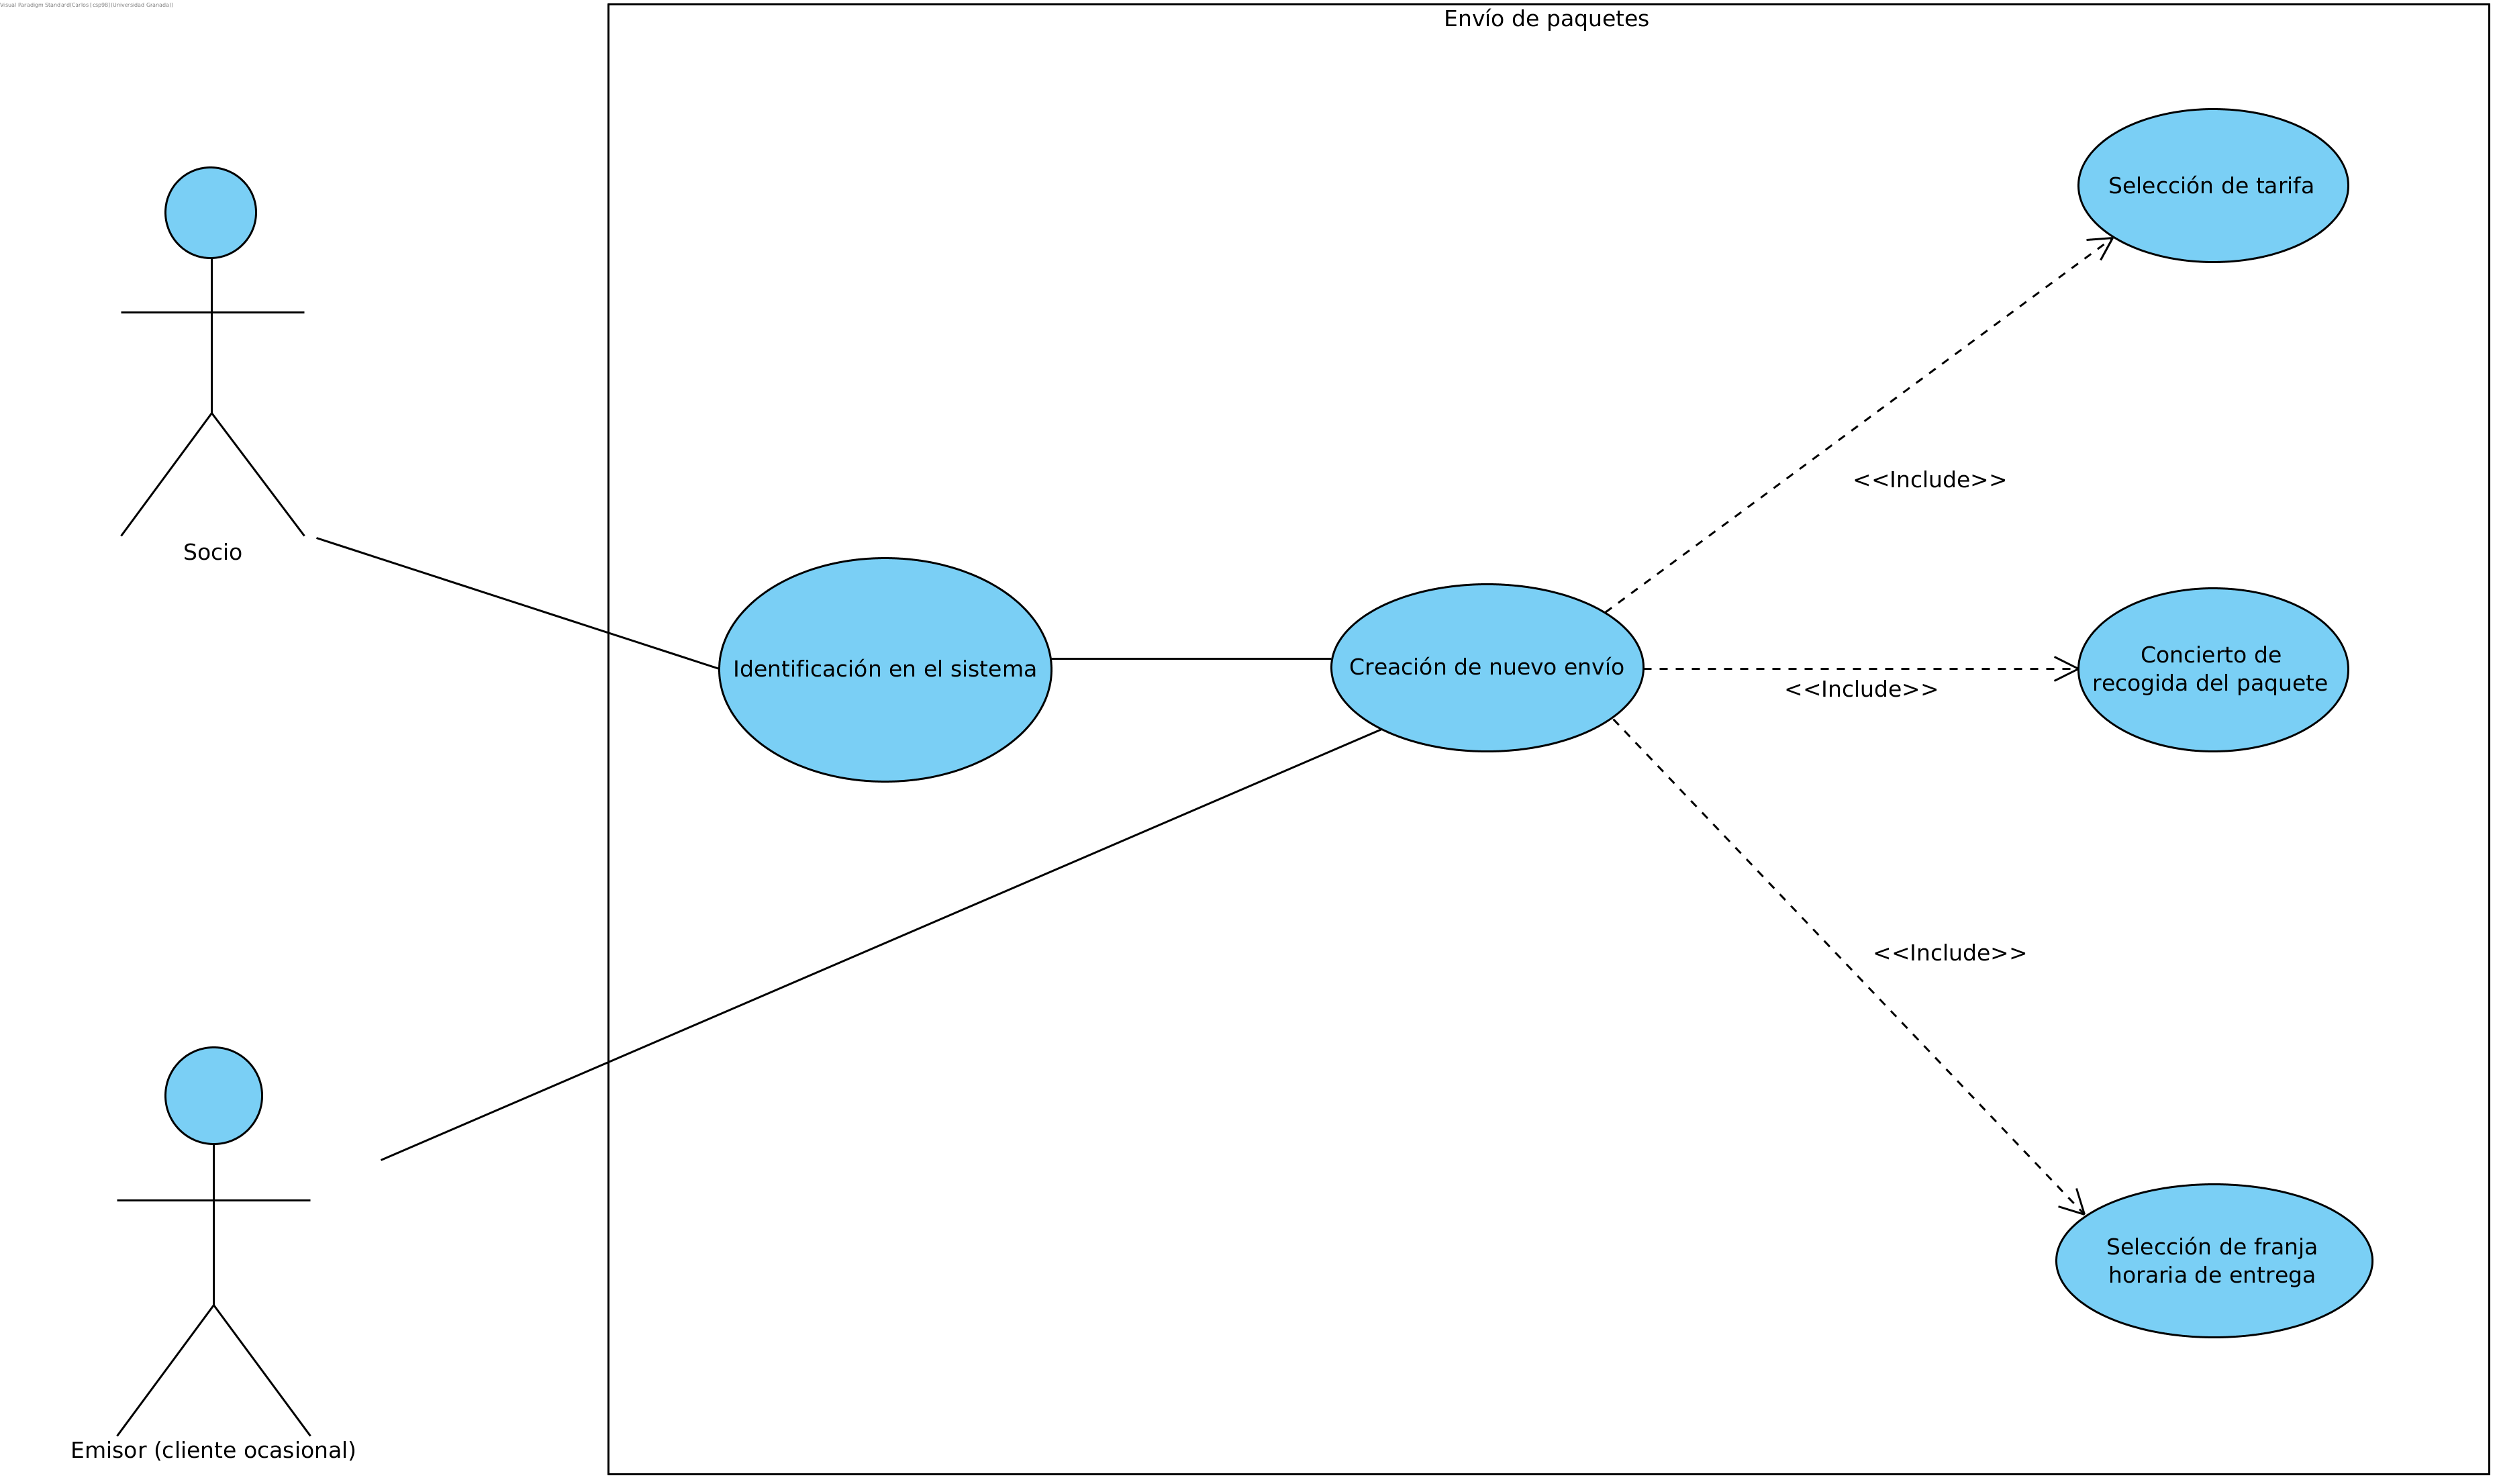
\includegraphics[scale=0.5]{enviar_paquete.png}
\caption{Enviar paquete}
\end{figure}

\begin{figure}[H]
\centering
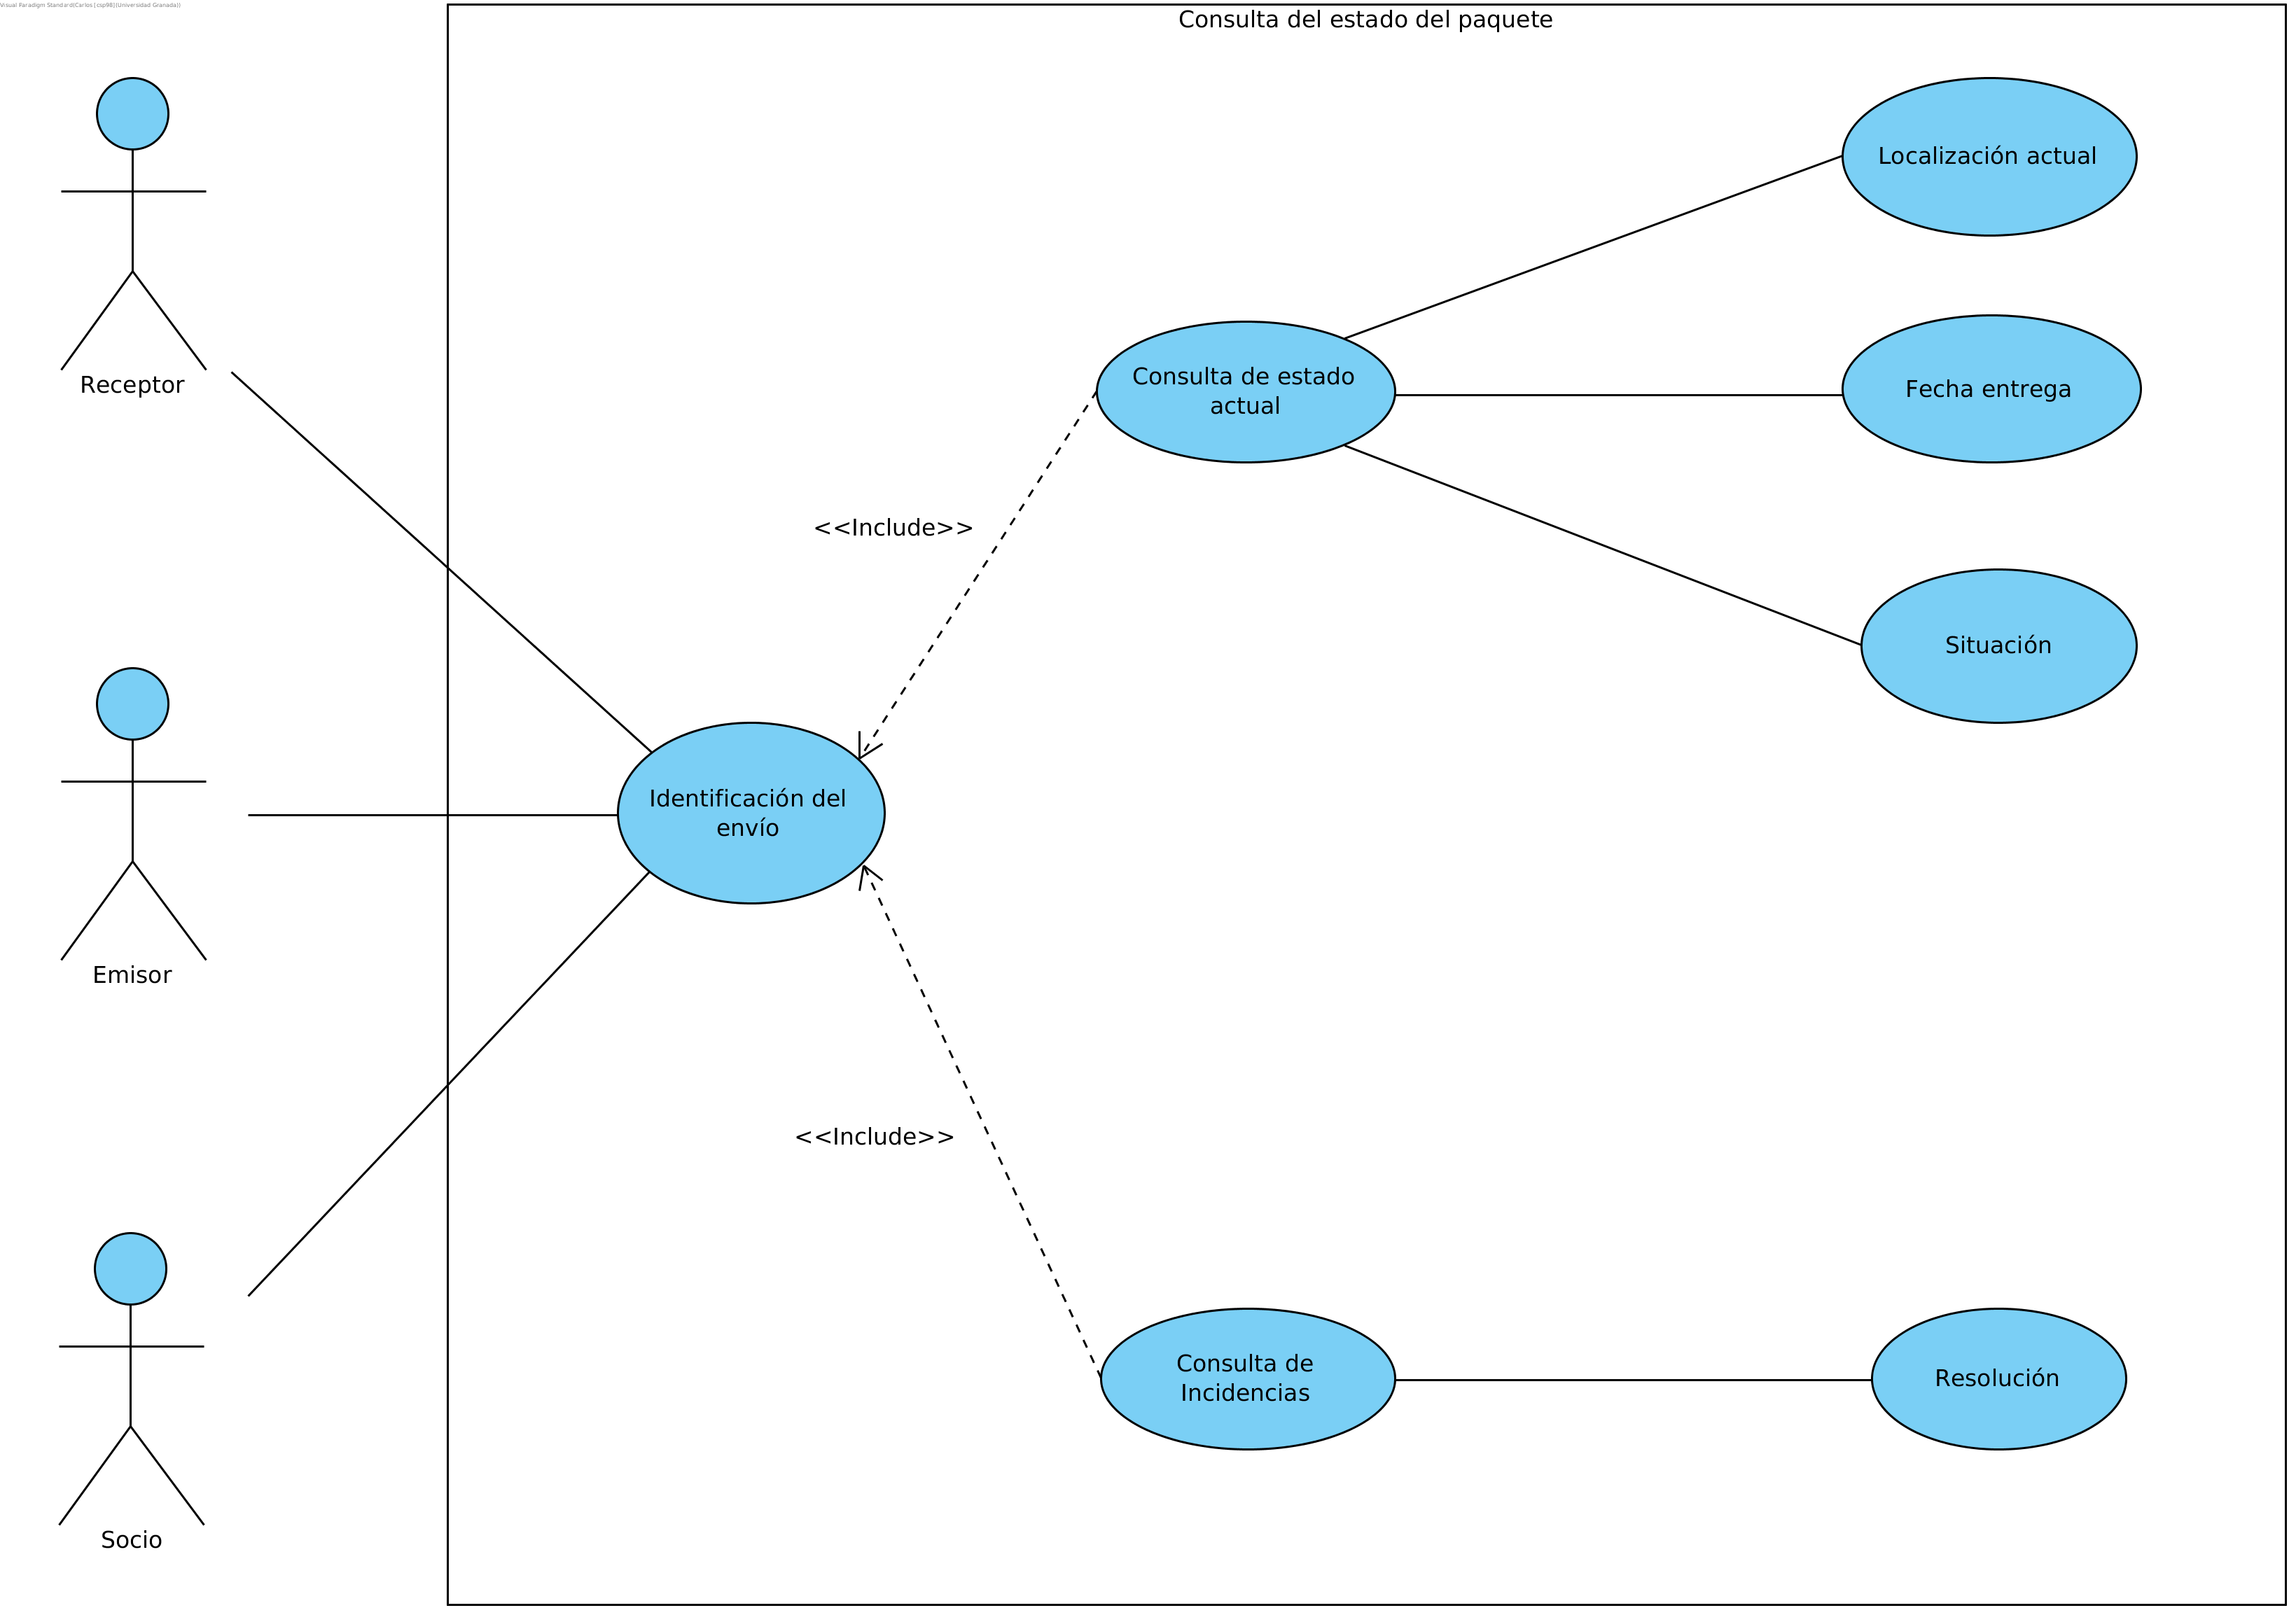
\includegraphics[scale=0.5]{consultar_estado.png}
\caption{Consultar estado del paquete}
\end{figure}

\begin{figure}[H]
\centering
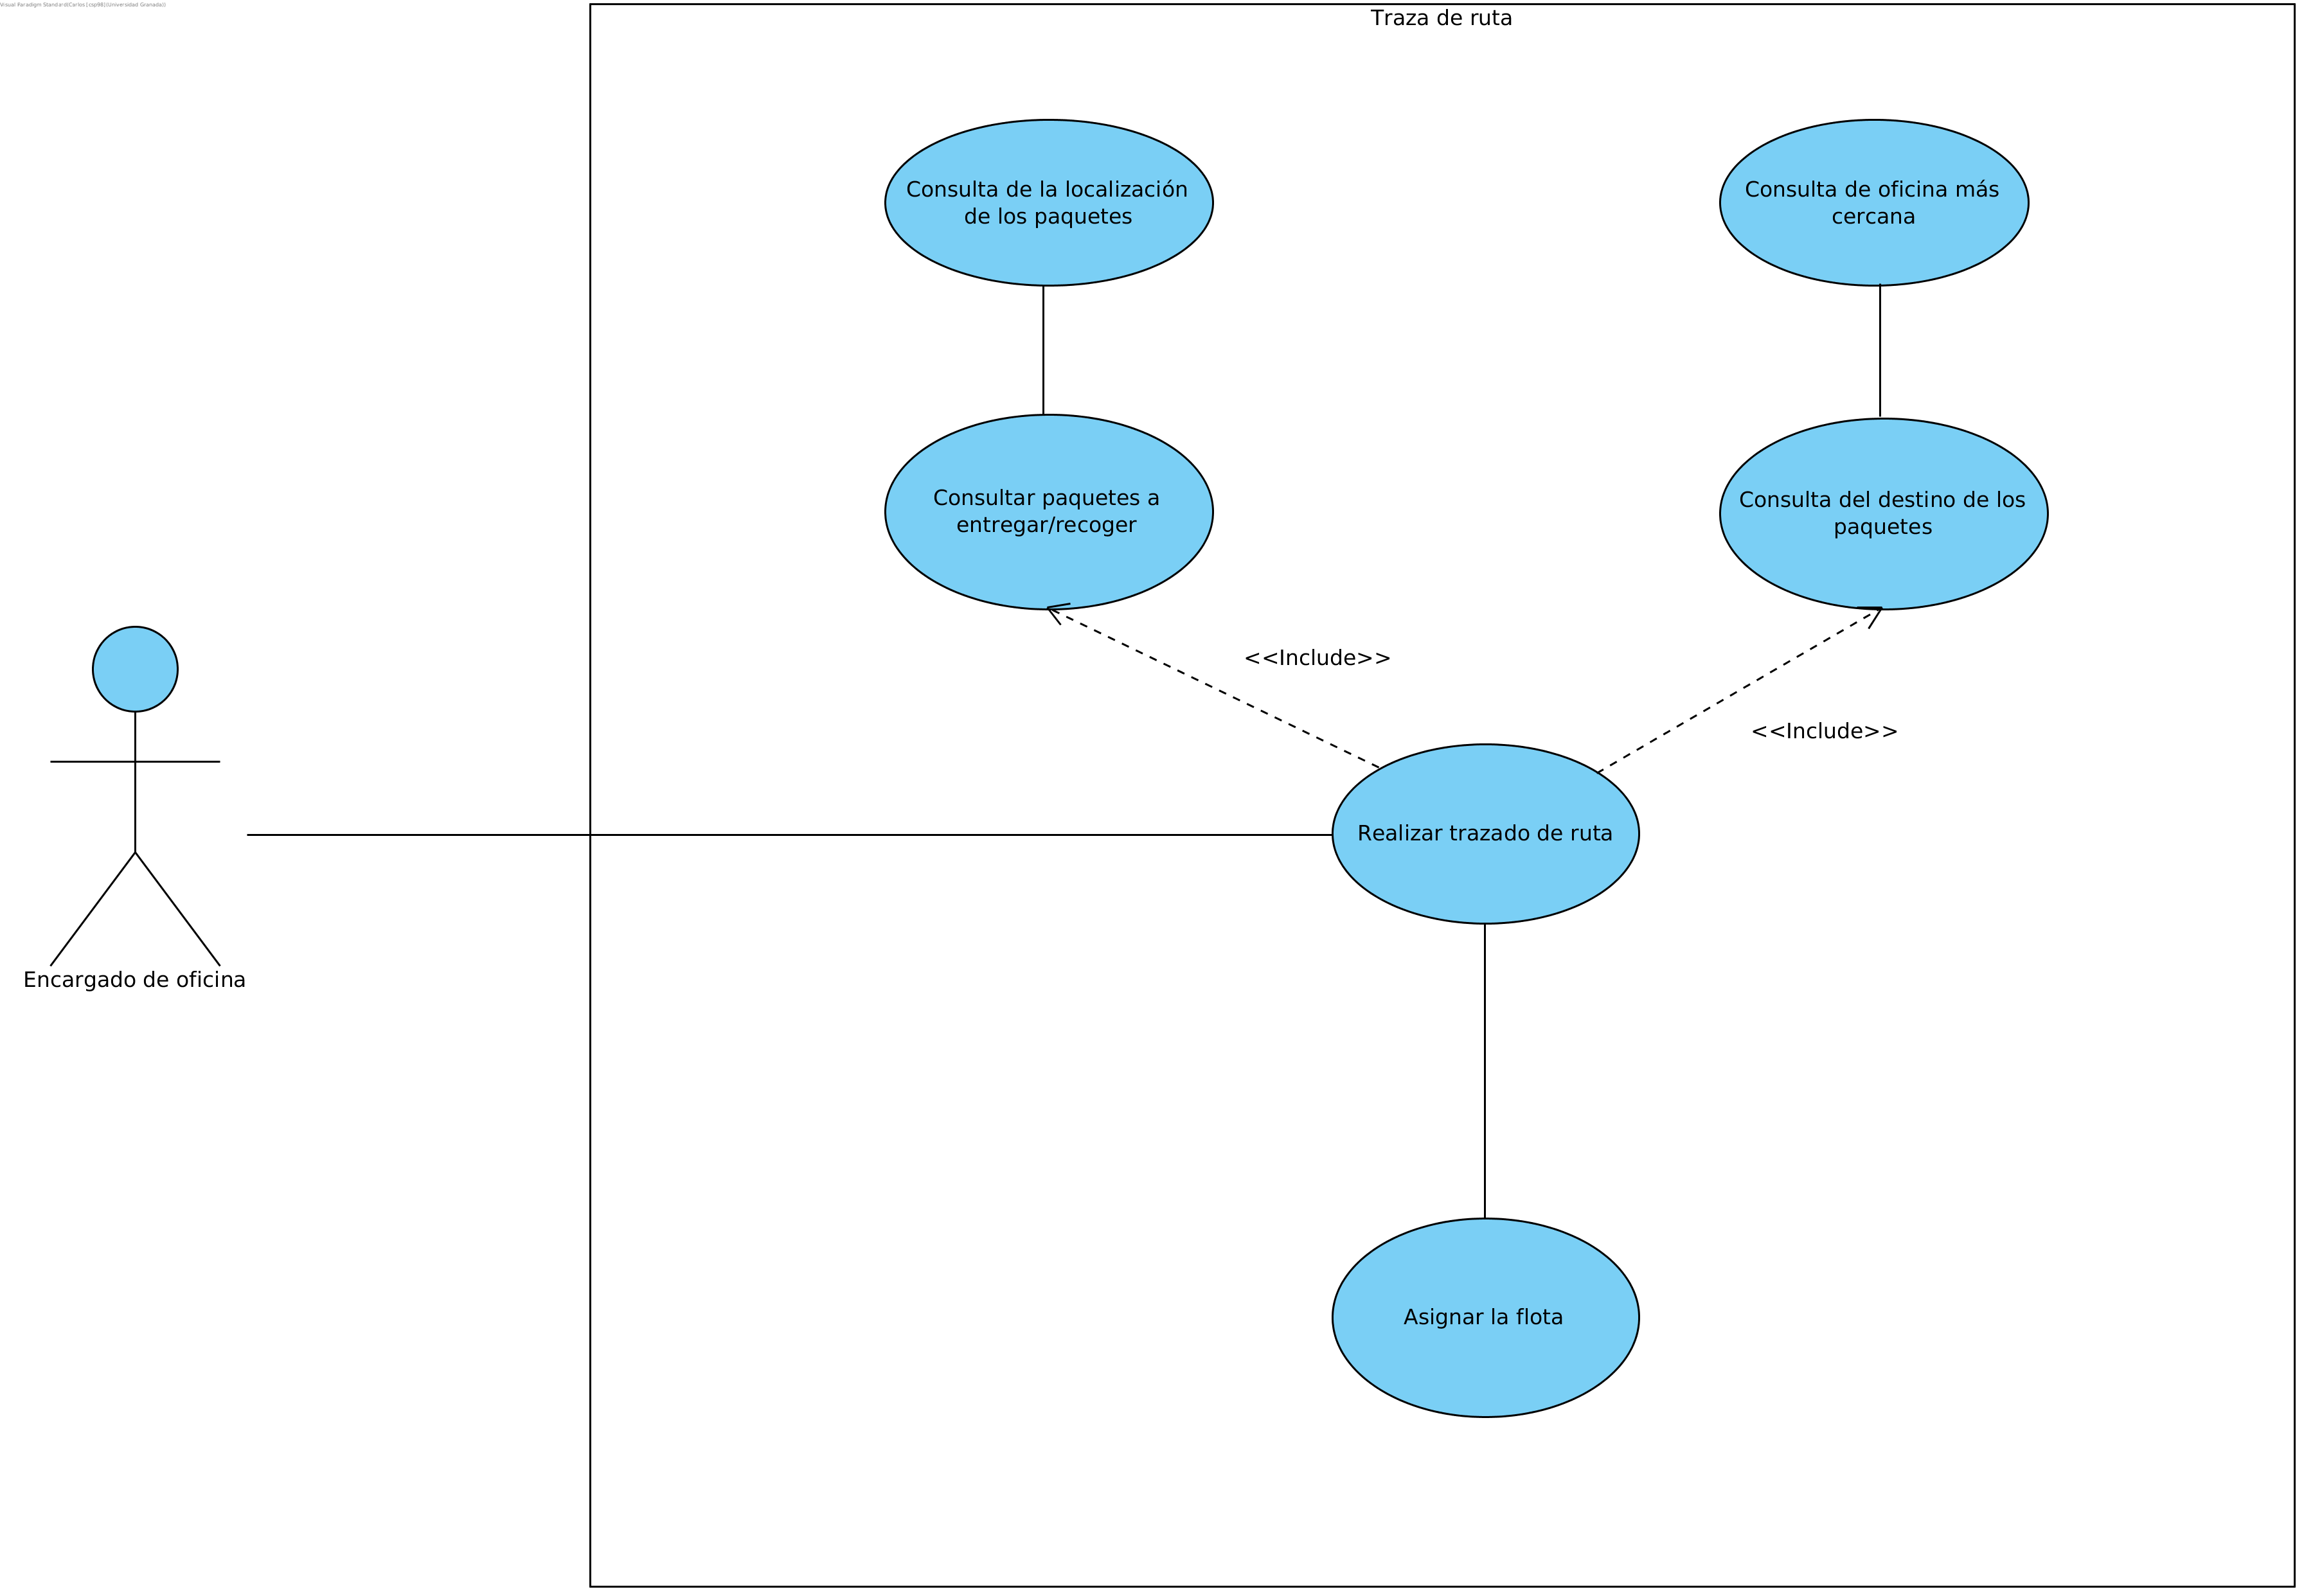
\includegraphics[scale=0.5]{trazar_ruta.png}
\caption{Trazar la ruta}
\end{figure}


\begin{figure}[H]
\centering
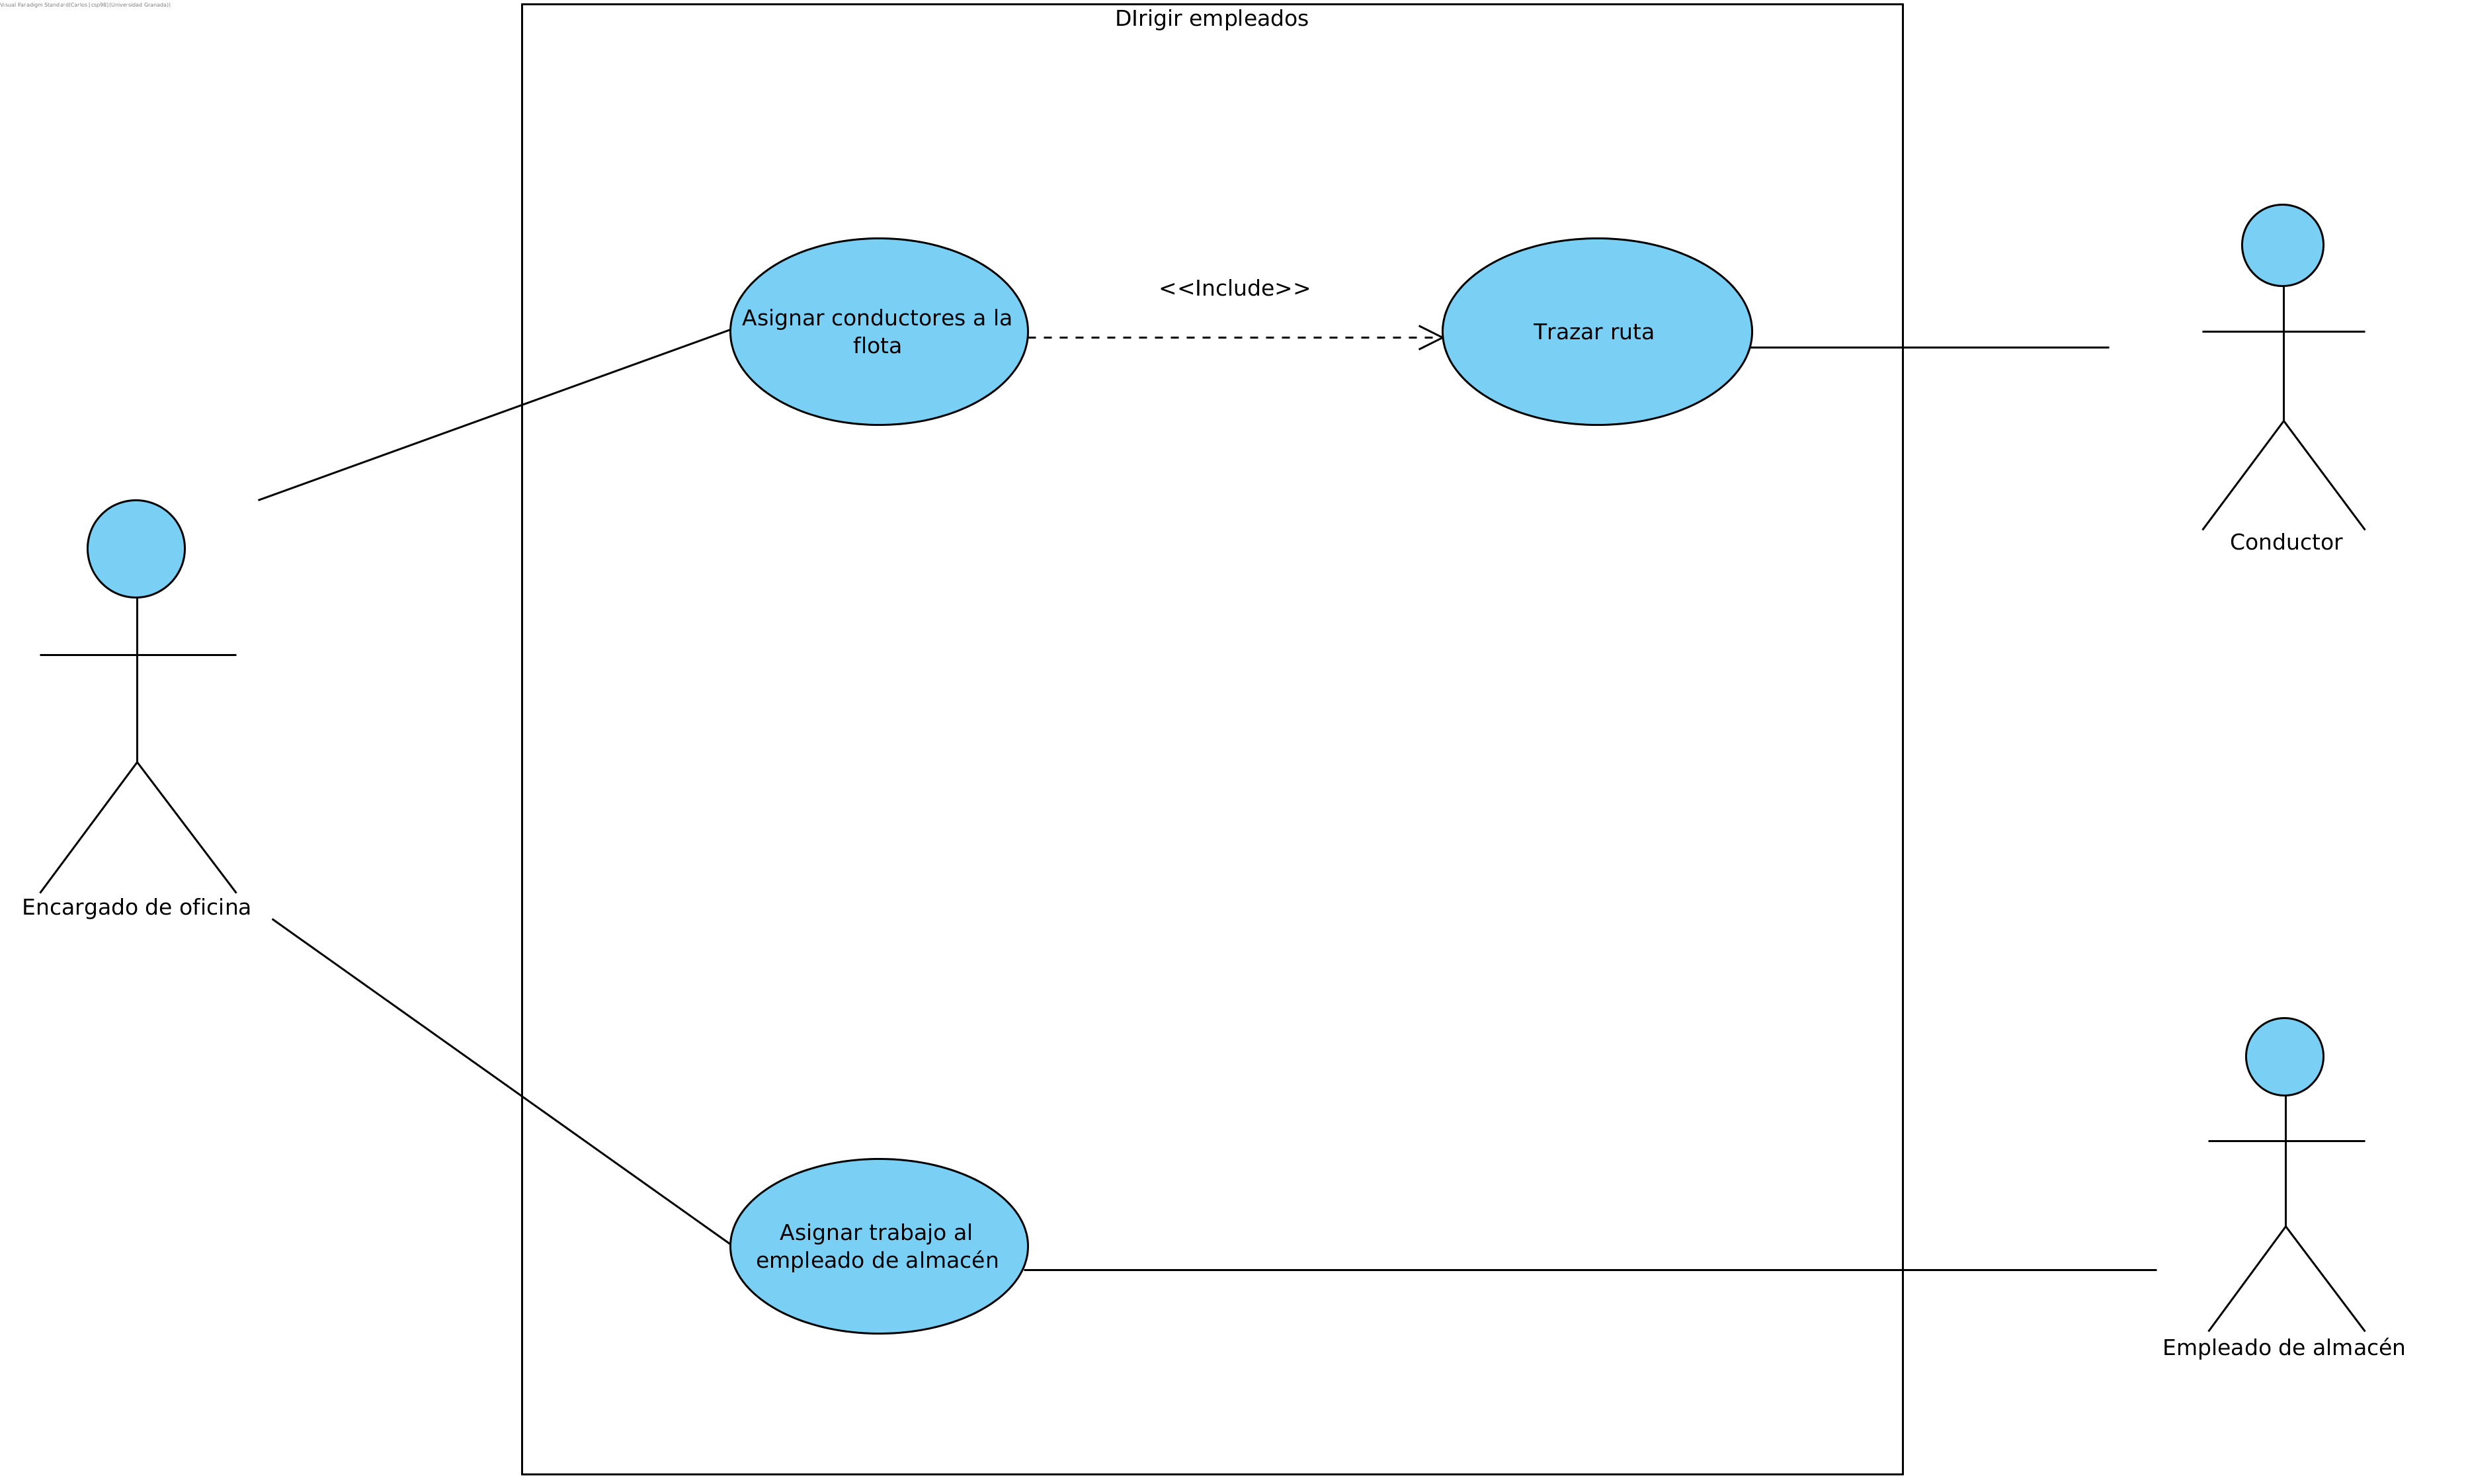
\includegraphics[scale=0.5]{dirigir_empleados.png}
\caption{Dirigir a los empleados}
\end{figure}


\begin{figure}[H]
\centering
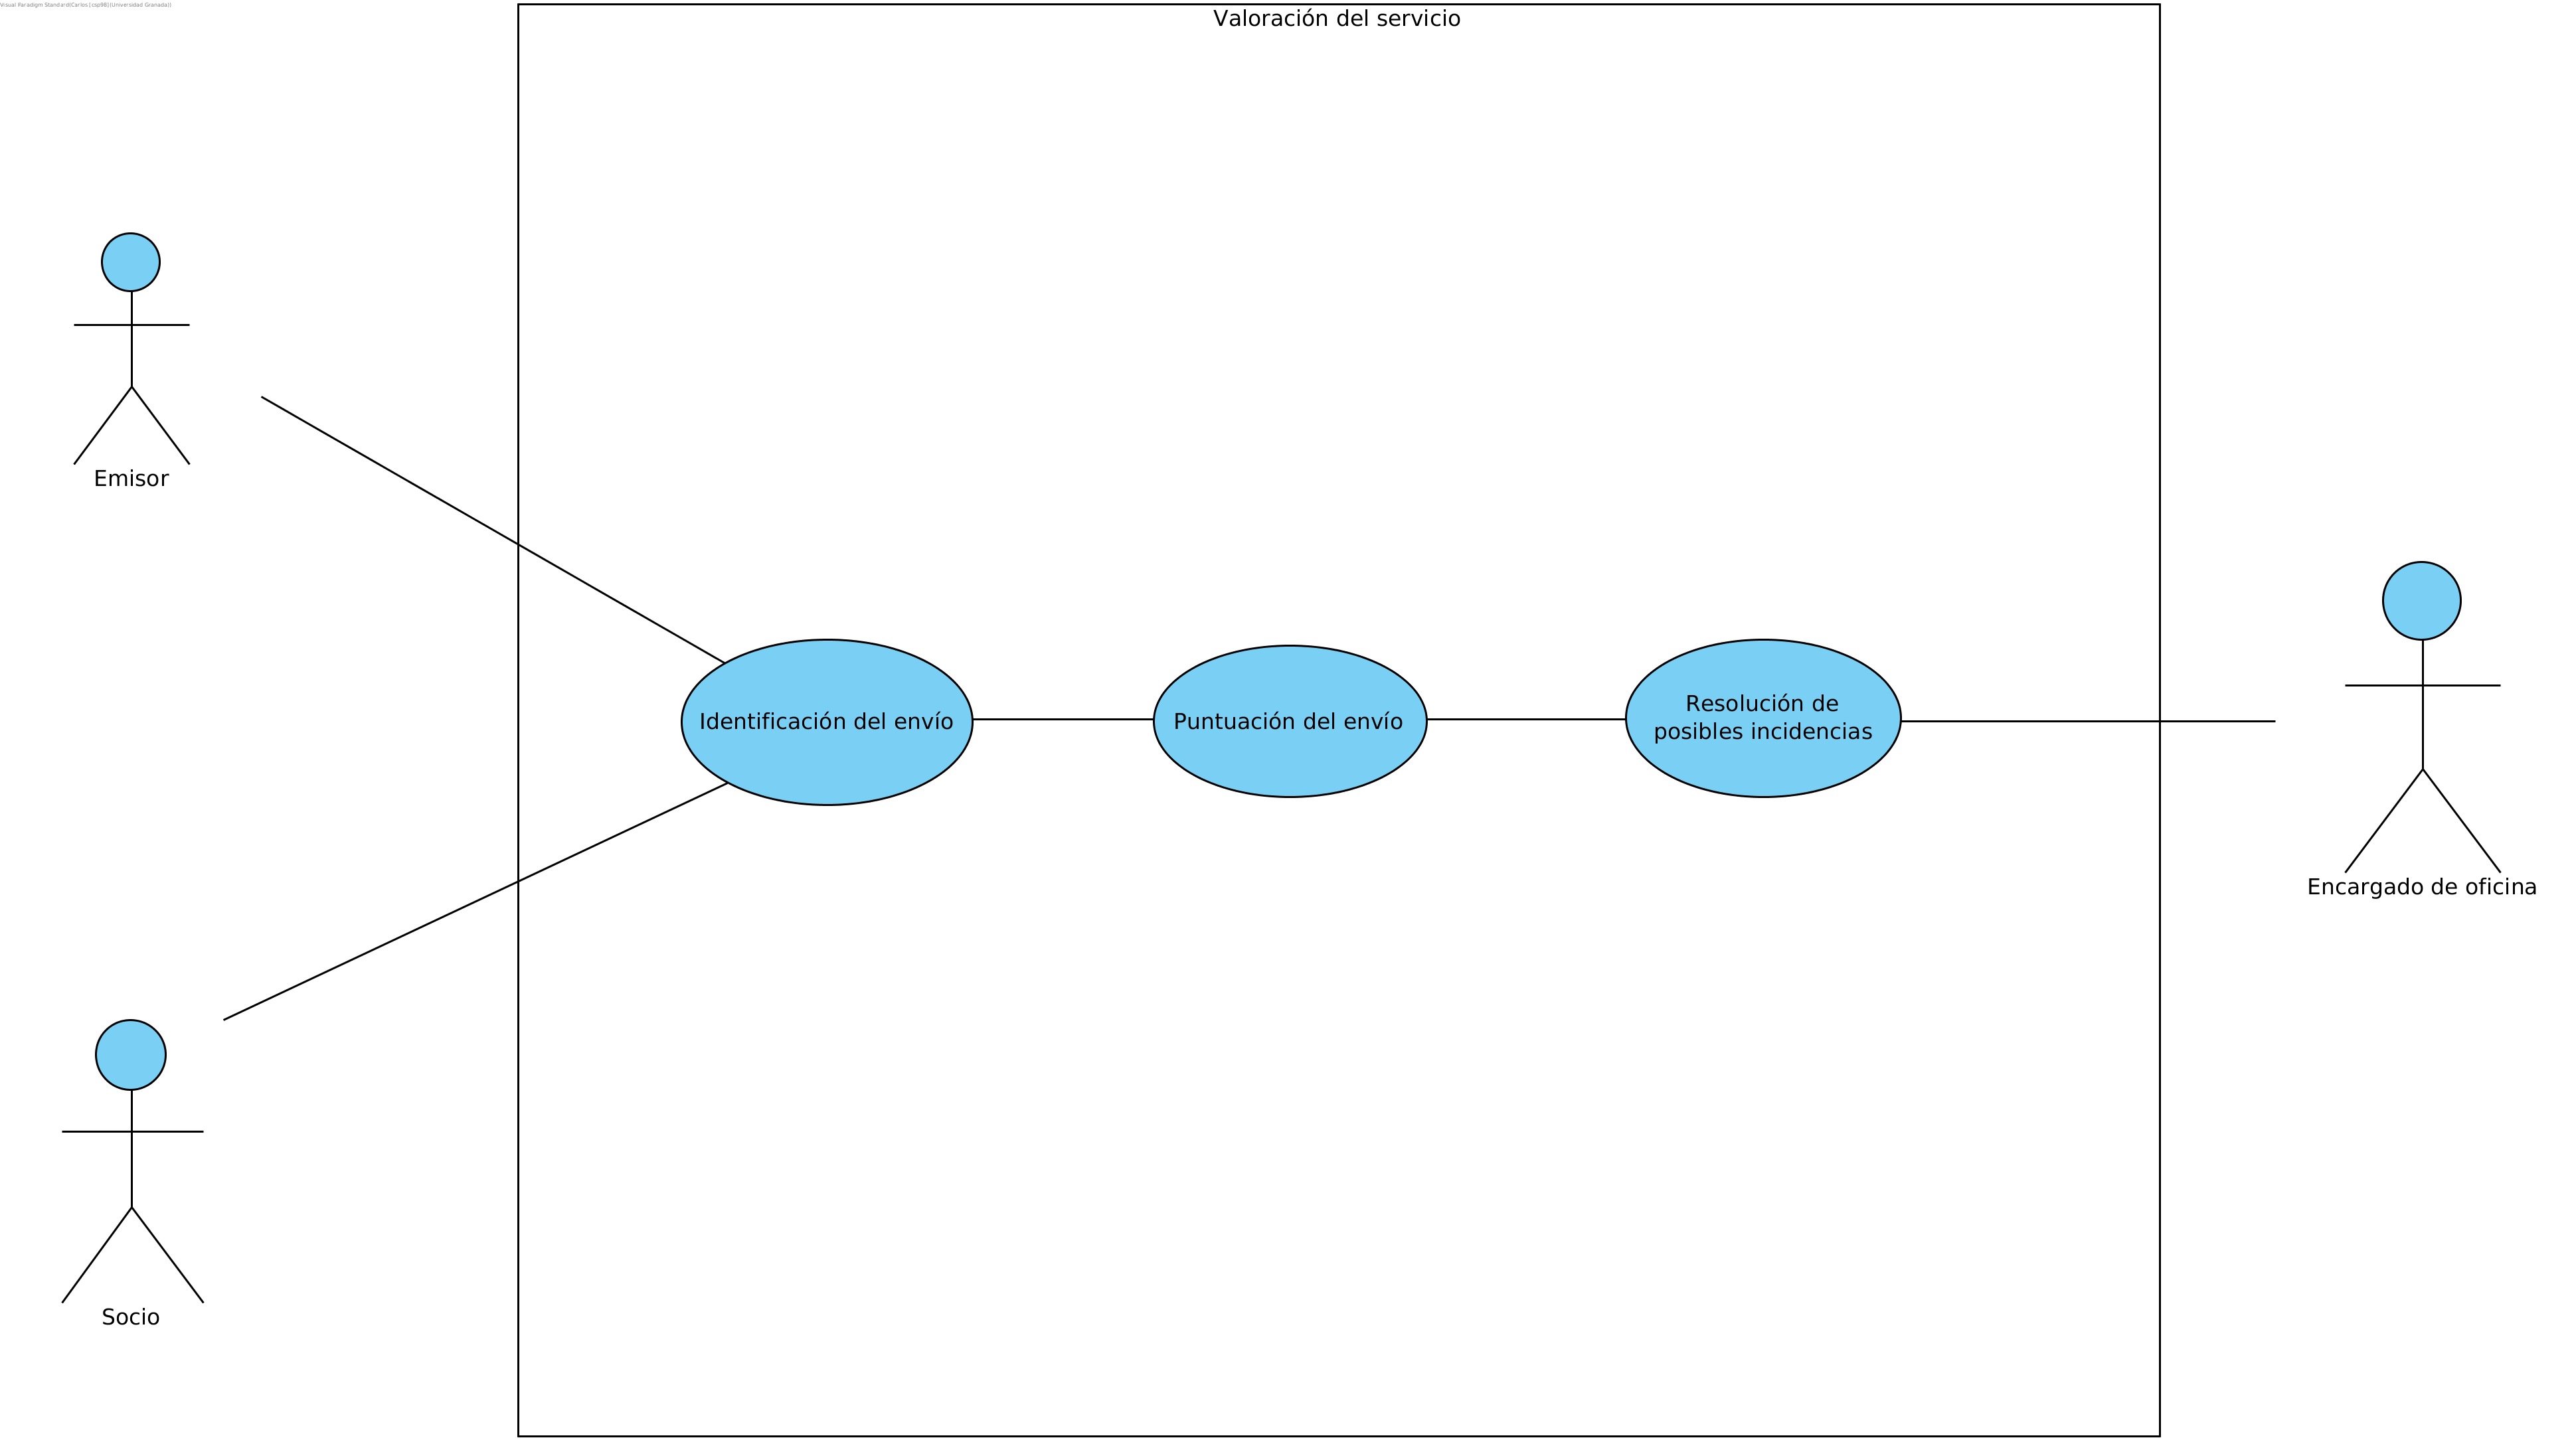
\includegraphics[scale=0.5]{valorar_servicio.png}
\caption{Valorar el servicio}
\end{figure}

\begin{figure}[H]
\centering
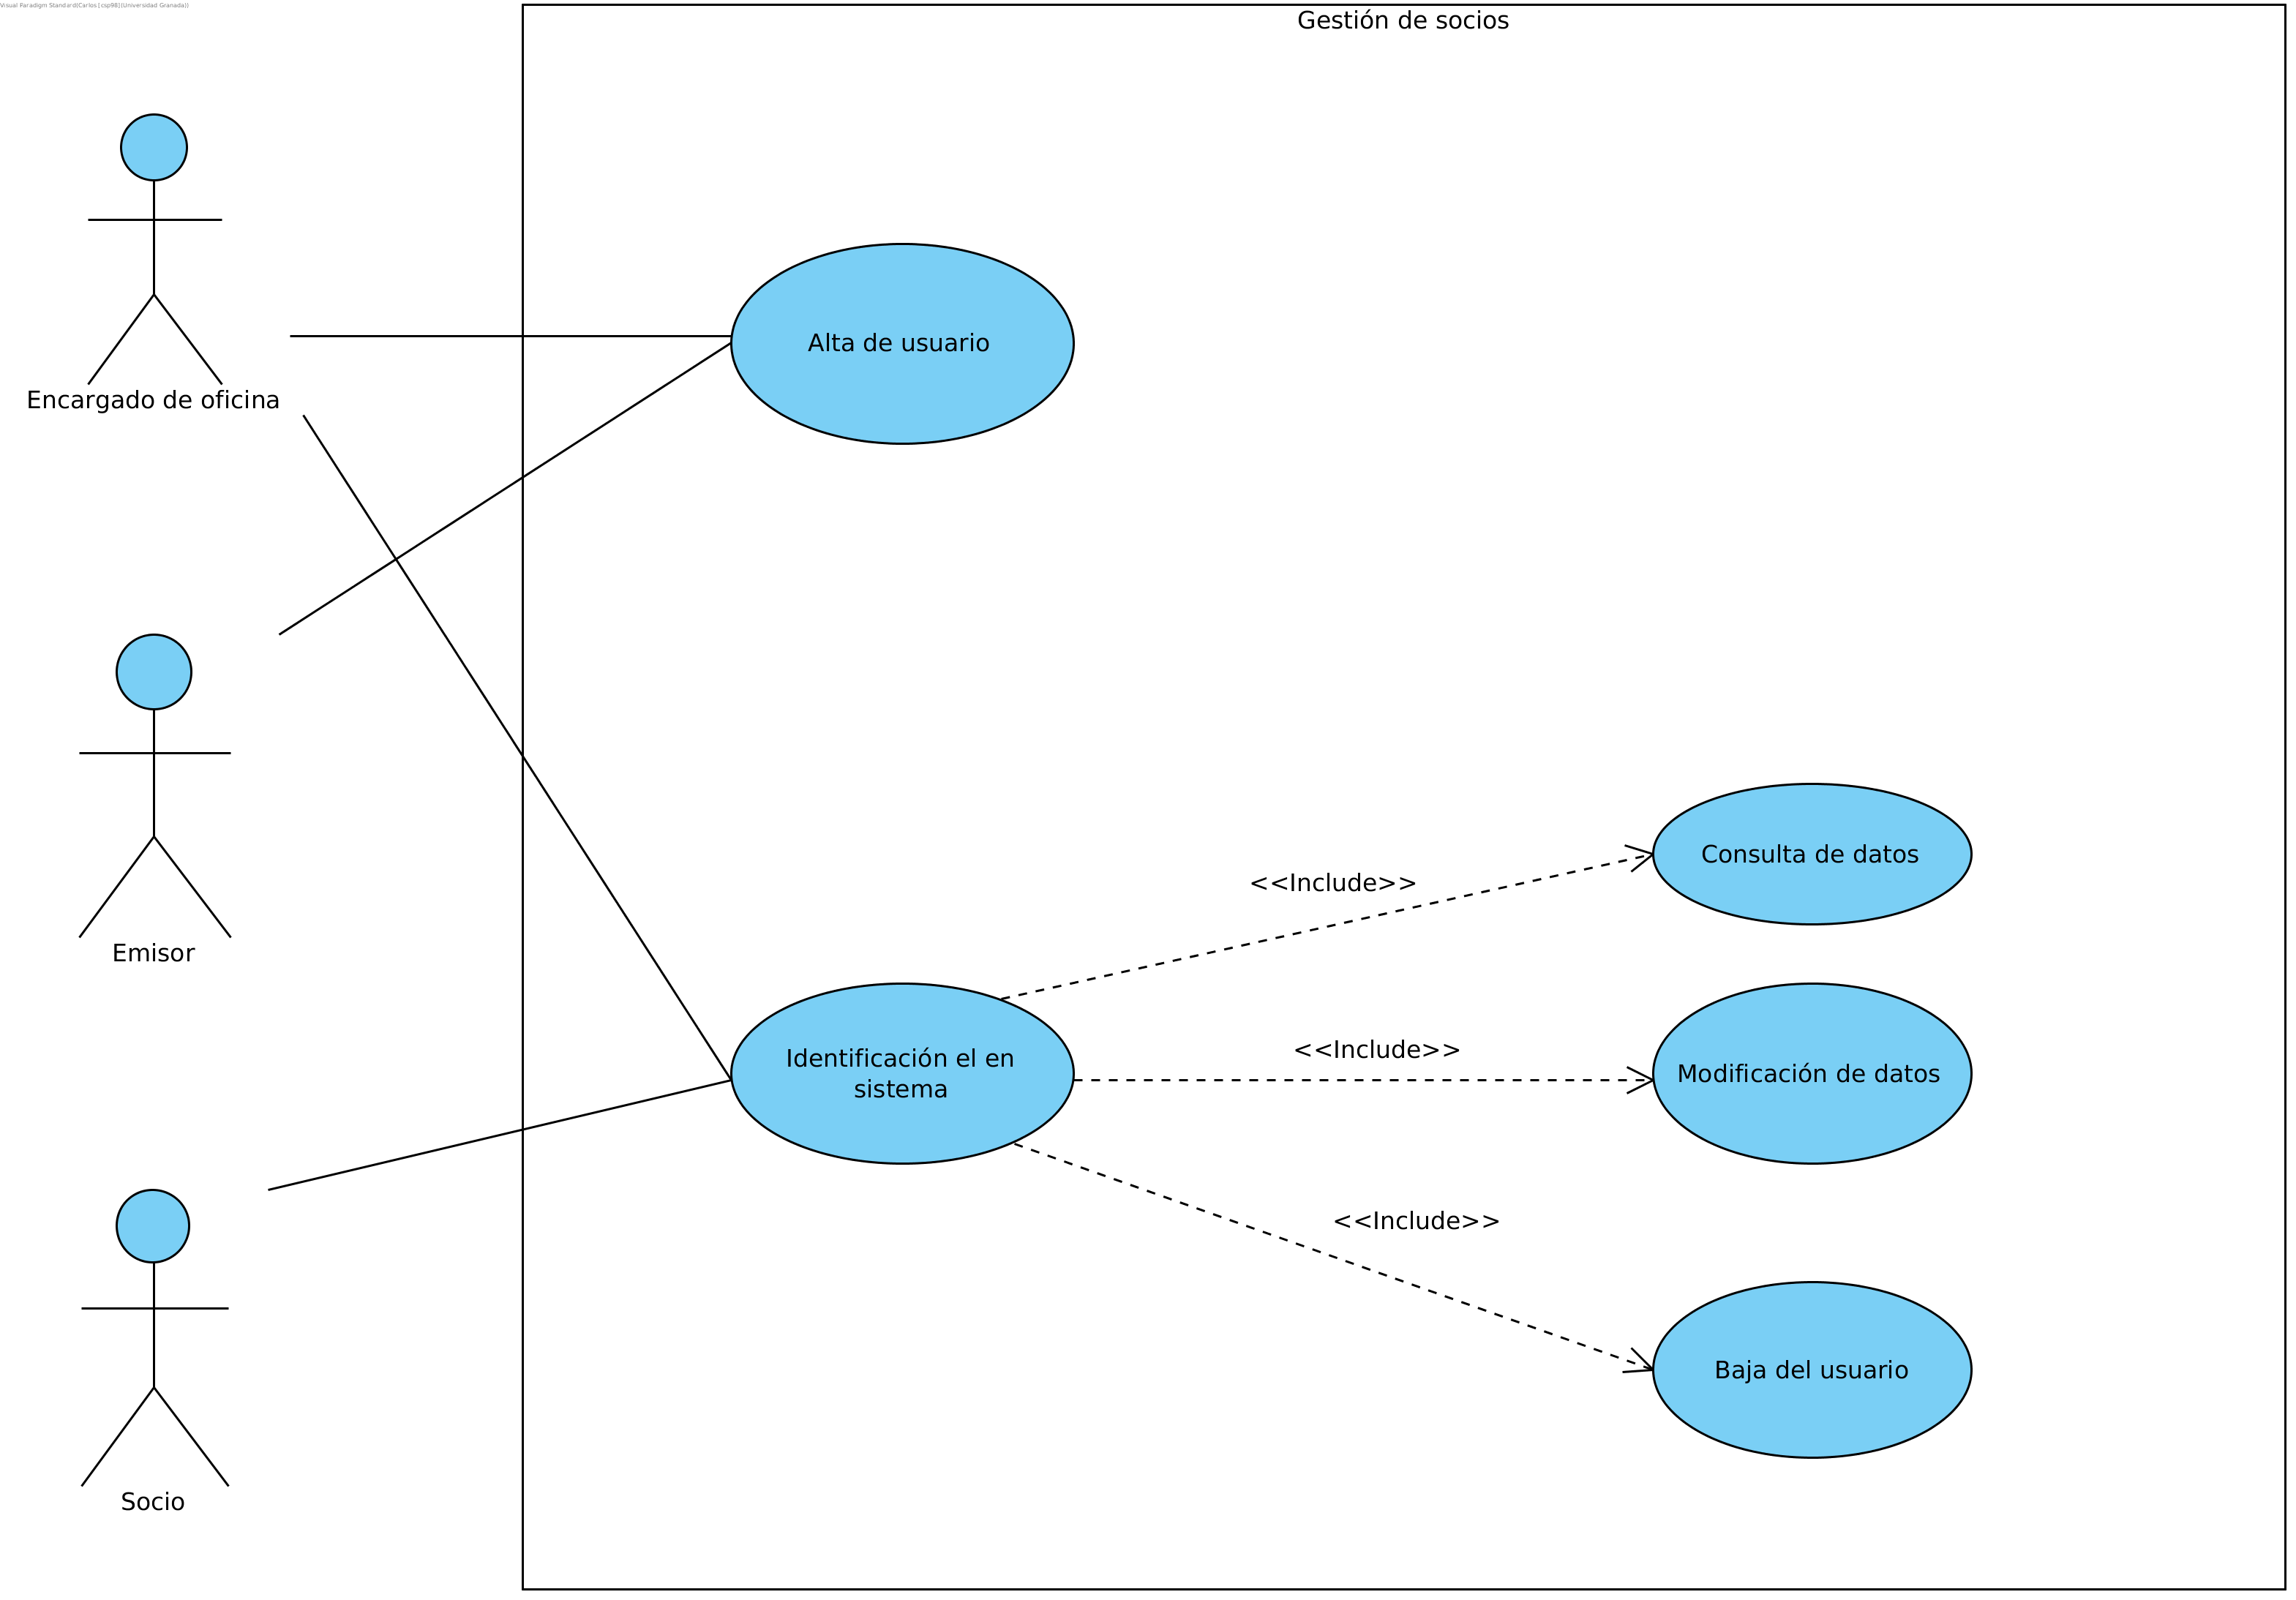
\includegraphics[scale=0.5]{gestion_socios.png}
\caption{Gestionar socios}
\end{figure}

\section{Diagrama de paquetes}

\begin{figure}[H]
\centering
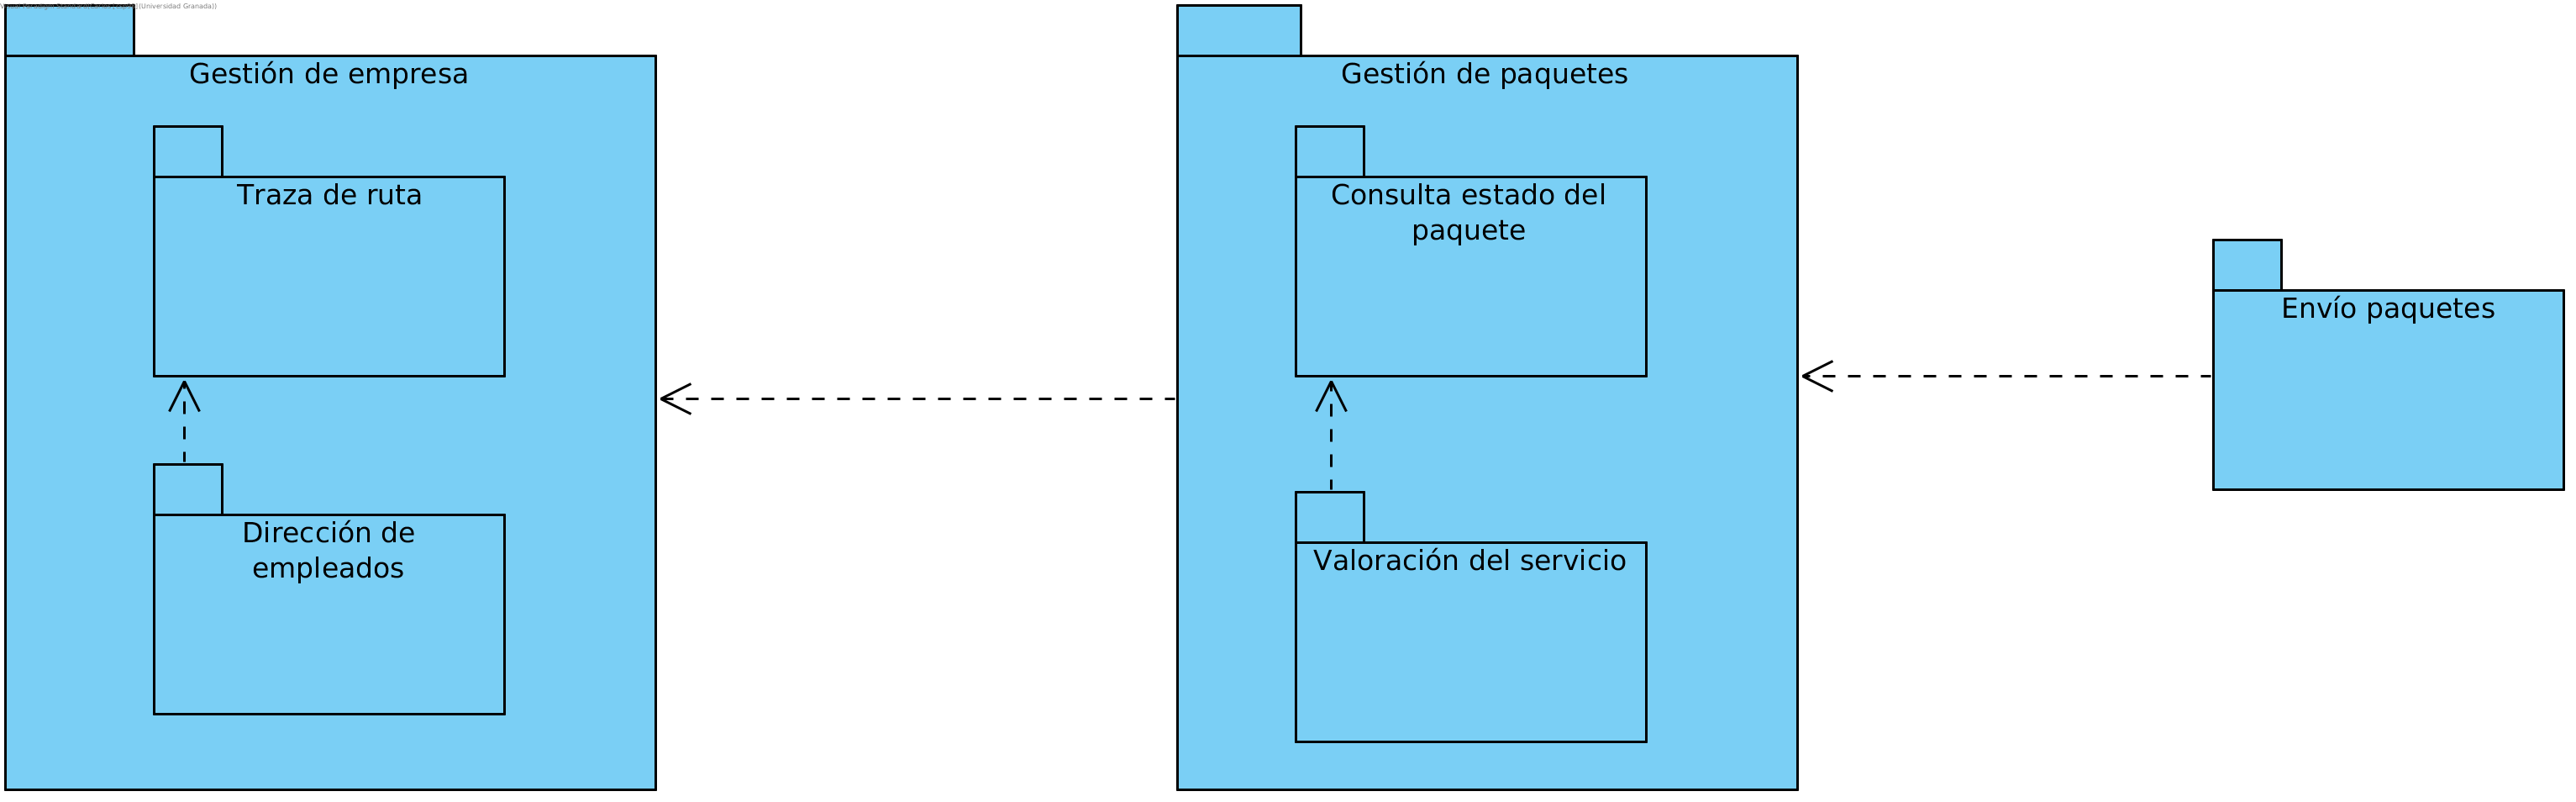
\includegraphics[scale=0.5]{paquetes.png}
\caption{Diagrama de paquetes}
\end{figure}

\section{Descripción de casos de uso a nivel general}

\subsection{José Miguel Pelegrina Pelegrina}

%%%%%%%%%%%CONSULTAR ESTADO DE PAQUETE%%%%%%%%%%%%%%%%

\begin{table}[H]
\centering
\begin{tabular}{|m{3cm}|m{4cm}|m{2cm}|m{2cm}|m{2cm}|m{1cm}|}
\hline
\textbf{Caso de uso} &  \multicolumn{4}{m{8cm}|}{Consultar el estado de un paquete} \vline &  \cellcolor{gray!40}CU2 \\
\hline
\textbf{Actores} & \multicolumn{5}{m{8cm}|}{Emisor, socio, receptor} \\
\hline
\textbf{Tipo} & \multicolumn{5}{m{8cm}|}{Secundario, Esencial} \\
\hline
\textbf{Referencias} &\multicolumn{5}{m{8cm}|}{CU-2.1} \\
\hline
\textbf{Precondición} & \multicolumn{5}{m{8cm}|}{-} \\
\hline
\textbf{Postcondición} & \multicolumn{5}{m{8cm}|}{-} \\
\hline
\textbf{Autor} & José Miguel Pelegrina Pelegrina & \textbf{Fecha} & 21/03/18 & \textbf{Versión} & 1.0 \\
\hline
\end{tabular}

\vspace{1cm}

\begin{tabular}{|m{16.2cm}|}
\hline
\textbf{Propósito} \\
\hline
Obtener la fecha de entrega de un paquete concreto \\
\hline
\end{tabular}

\vspace{1cm}

\begin{tabular}{|m{16.2cm}|}
\hline
\textbf{Resumen} \\
\hline
Un cliente solicita la información de un paquete, mostrando su fecha de entrega. \\
\hline
\end{tabular}

\caption{Consultar el estado de un paquete}
\label{cu:2}
\end{table}
 
%%%%%%%%%%%%%%%%%%%%%%%%%%%%%%%%%%%%%%%%%%%%%%%%%

%%%%%%%%%%%%GESTIÓN DE SOCIOS%%%%%%%%%%%%%%%%%%%%


\begin{table}[H]
\centering
\begin{tabular}{|m{3cm}|m{4cm}|m{2cm}|m{2cm}|m{2cm}|m{1cm}|}
\hline
\textbf{Caso de uso} &  \multicolumn{4}{m{8cm}|}{Alta de socio} \vline &  \cellcolor{gray!40}CU6.1 \\
\hline
\textbf{Actores} & \multicolumn{5}{m{8cm}|}{Cliente, Empleado de oficina} \\
\hline
\textbf{Tipo} & \multicolumn{5}{m{8cm}|}{Primario, Esencial} \\
\hline
\textbf{Referencias} &\multicolumn{5}{m{8cm}|}{-} \\
\hline
\textbf{Precondición} & \multicolumn{5}{m{8cm}|}{-} \\
\hline
\textbf{Postcondición} & \multicolumn{5}{m{8cm}|}{El nuevo socio puede acceder al sistema mediante su DNI y una clave} \\
\hline
\textbf{Autor} & Jose Miguel Pelegrina Pelegrina & \textbf{Fecha} & 21/03/18 & \textbf{Versión} & 1.0 \\
\hline
\end{tabular}

\vspace{1cm}

\begin{tabular}{|m{16.2cm}|}
\hline
\textbf{Propósito} \\
\hline
Un cliente pide que se le haga socio. \\
\hline
\end{tabular}

\vspace{1cm}

\begin{tabular}{|m{16.2cm}|}
\hline
\textbf{Resumen} \\
\hline
El empleado le hace socio haciendo que pueda entrar en el sistema con sus credenciales. \\
\hline
\end{tabular}

\caption{Alta de Socio}
\label{cu:6}
\end{table}

\begin{table}[H]
\centering
\begin{tabular}{|m{3cm}|m{4cm}|m{2cm}|m{2cm}|m{2cm}|m{1cm}|}
\hline
\textbf{Caso de uso} &  \multicolumn{4}{m{8cm}|}{Baja de socio} \vline &  \cellcolor{gray!40}CU6.2 \\
\hline
\textbf{Actores} & \multicolumn{5}{m{8cm}|}{Socio, Empleado de oficina} \\
\hline
\textbf{Tipo} & \multicolumn{5}{m{8cm}|}{Secundario, Esencial} \\
\hline
\textbf{Referencias} &\multicolumn{5}{m{8cm}|}{-} \\
\hline
\textbf{Precondición} & \multicolumn{5}{m{8cm}|}{-} \\
\hline
\textbf{Postcondición} & \multicolumn{5}{m{8cm}|}{-} \\
\hline
\textbf{Autor} & José Miguel Pelegrina Pelegrina & \textbf{Fecha} & 21/03/18 & \textbf{Versión} & 1.0 \\
\hline
\end{tabular}

\vspace{1cm}

\begin{tabular}{|m{16.2cm}|}
\hline
\textbf{Propósito} \\
\hline
Representa la acción por parte de un socio de pedir la baja de la empresa \\
\hline
\end{tabular}

\vspace{1cm}

\begin{tabular}{|m{16.2cm}|}
\hline
\textbf{Resumen} \\
\hline
El socio pide al empleado de oficina que quiere darse de baja de la empresa y el empleado elimina sus datos del sistema. \\
\hline
\end{tabular}

\caption{Baja de Socio}
\end{table}

\begin{table}[H]
\centering
\begin{tabular}{|m{3cm}|m{4cm}|m{2cm}|m{2cm}|m{2cm}|m{1cm}|}
\hline
\textbf{Caso de uso} &  \multicolumn{4}{m{8cm}|}{Consulta de socios} \vline &  \cellcolor{gray!40}CU6.3 \\
\hline
\textbf{Actores} & \multicolumn{5}{m{8cm}|}{Empleado de oficina} \\
\hline
\textbf{Tipo} & \multicolumn{5}{m{8cm}|}{Secundario, Esencial} \\
\hline
\textbf{Referencias} &\multicolumn{5}{m{8cm}|}{-} \\
\hline
\textbf{Precondición} & \multicolumn{5}{m{8cm}|}{-} \\
\hline
\textbf{Postcondición} & \multicolumn{5}{m{8cm}|}{-} \\
\hline
\textbf{Autor} & José Miguel Pelegrina Pelegrina & \textbf{Fecha} & 21/03/18 & \textbf{Versión} & 1.0 \\
\hline
\end{tabular}

\vspace{1cm}

\begin{tabular}{|m{16.2cm}|}
\hline
\textbf{Propósito} \\
\hline
Obtener información sobre los datos personales de un socio. \\
\hline
\end{tabular}

\vspace{1cm}

\begin{tabular}{|m{16.2cm}|}
\hline
\textbf{Resumen} \\
\hline
El empleado de oficina solicita información sobre un socio y el sistema le proporciona la información que posee sobre el mismo. \\
\hline
\end{tabular}

\caption{Consulta de Socio}
\end{table}

\begin{table}[H]
\centering
\begin{tabular}{|m{3cm}|m{4cm}|m{2cm}|m{2cm}|m{2cm}|m{1cm}|}
\hline
\textbf{Caso de uso} &  \multicolumn{4}{m{8cm}|}{Modificación de socio} \vline &  \cellcolor{gray!40}CU6.4 \\
\hline
\textbf{Actores} & \multicolumn{5}{m{8cm}|}{Socio(I),Empleado de Oficina} \\
\hline
\textbf{Tipo} & \multicolumn{5}{m{8cm}|}{Secundario, Esencial} \\
\hline
\textbf{Referencias} &\multicolumn{5}{m{8cm}|}{-} \\
\hline
\textbf{Precondición} & \multicolumn{5}{m{8cm}|}{-} \\
\hline
\textbf{Postcondición} & \multicolumn{5}{m{8cm}|}{-} \\
\hline
\textbf{Autor} & José Miguel Pelegrina Pelegrina & \textbf{Fecha} & 21/03/18 & \textbf{Versión} & 1.0 \\
\hline
\end{tabular}

\vspace{1cm}

\begin{tabular}{|m{16.2cm}|}
\hline
\textbf{Propósito} \\
\hline
Modificar alguno de los datos que la empresa posee sobre un socio. \\
\hline
\end{tabular}

\vspace{1cm}

\begin{tabular}{|m{16.2cm}|}
\hline
\textbf{Resumen} \\
\hline
El socio solicita al empleado el cambio de alguno de sus datos personales, suministra los nuevos datos y se realizan los cambios pertinentes. \\
\hline
\end{tabular}

\caption{Modificación de Socio}
\end{table}


%%%%%%%%%%%%%%%%%%%%%%%%%%%%%%%%%%%%%%%%%%%%%%%%%

\subsection{José Baena Cobos}

%%%%%%%%%%TRAZAR RUTA%%%%%%%%%%

\begin{table}[H]
\centering
\begin{tabular}{|m{3cm}|m{4cm}|m{2cm}|m{2cm}|m{2cm}|m{1cm}|}
\hline
\textbf{Caso de uso} &  \multicolumn{4}{m{8cm}|}{Trazar ruta} \vline &  \cellcolor{gray!40}CU3 \\
\hline
\textbf{Actores} & \multicolumn{5}{m{8cm}|}{Encargado de oficina} \\
\hline
\textbf{Tipo} & \multicolumn{5}{m{8cm}|}{Primario y esencial} \\
\hline
\textbf{Referencias} &\multicolumn{5}{m{8cm}|}{-} \\
\hline
\textbf{Precondición} & \multicolumn{5}{m{8cm}|}{Tener listos los pedidos a realizar en el día} \\
\hline
\textbf{Postcondición} & \multicolumn{5}{m{8cm}|}{Las furgonetas tendrán una ruta asignada con unas tarea concretas} \\
\hline
\textbf{Autor} & José Baena Cobos & \textbf{Fecha} & 20/03/18 & \textbf{Versión} & 2.0 \\
\hline
\end{tabular}

\vspace{1cm}

\begin{tabular}{|m{16.2cm}|}
\hline
\textbf{Propósito} \\
\hline
Gestionar la ruta que seguirán las furgonetas de reparto para recoger y enviar los paquetes. \\
\hline
\end{tabular}

\vspace{1cm}

\begin{tabular}{|m{16.2cm}|}
\hline
\textbf{Resumen} \\
\hline
Se consultan los puntos por donde deben pasar las furgonetas de transporte para trazar la ruta más eficiente. \\
\hline
\end{tabular}

\caption{Trazar ruta}
\label{cu:3}
\end{table}

%%%%%%%%%%%%%%%%%%%%%%%%%%%%%%%

%%%%%%%%%VALORAR SERVICIO%%%%%%


\begin{table}[H]
\centering
\begin{tabular}{|m{3cm}|m{4cm}|m{2cm}|m{2cm}|m{2cm}|m{1cm}|}
\hline
\textbf{Caso de uso} &  \multicolumn{4}{m{8cm}|}{Valorar el servicio} \vline &  \cellcolor{gray!40}CU5 \\
\hline
\textbf{Actores} & \multicolumn{5}{m{8cm}|}{\begin{enumerate}
		\item Socio o emisor.
		\item Encargado de oficina.
	\end{enumerate}} \\
\hline
\textbf{Tipo} & \multicolumn{5}{m{8cm}|}{No obligatorio y secundario} \\
\hline
\textbf{Referencias} &\multicolumn{5}{m{8cm}|}{-} \\
\hline
\textbf{Precondición} & \multicolumn{5}{m{8cm}|}{Haber realizado un pedido} \\
\hline
\textbf{Postcondición} & \multicolumn{5}{m{8cm}|}{-} \\
\hline
\textbf{Autor} & José Baena Cobos & \textbf{Fecha} & 20/03/18 & \textbf{Versión} & 2.0 \\
\hline
\end{tabular}

\vspace{1cm}

\begin{tabular}{|m{16.2cm}|}
\hline
\textbf{Propósito} \\
\hline
Resolver las incidencias de los clientes a la vez que se mejora la calidad del servicio de cara a futuros trabajos. \\
\hline
\end{tabular}

\vspace{1cm}

\begin{tabular}{|m{16.2cm}|}
\hline
\textbf{Resumen} \\
\hline
Tras realizar un pedido, el cliente tiene la posibilidad de dejar una reseña o incidencia sobre su pedido. En caso de que se trate de una incidencia, la empresa evaluará la situación y le buscará una solución. \\
\hline
\end{tabular}

\caption{Valorar el servicio}
\label{cu:5}
\end{table}


%%%%%%%%%%%%%%%%%%%%%%%%%%%%%%%
\subsection{Carlos Sánchez Páez}

%%%%%%%%%%%ENVIAR PAQUETE%%%%%%%%%%%%%%%%
\begin{table}[H]
\centering
\begin{tabular}{|m{3cm}|m{4cm}|m{2cm}|m{2cm}|m{2cm}|m{1cm}|}
\hline
\textbf{Caso de uso} &  \multicolumn{4}{m{8cm}|}{Enviar paquete} \vline &  \cellcolor{gray!40}CU1 \\
\hline
\textbf{Actores} & \multicolumn{5}{m{8cm}|}{Socio o emisor} \\
\hline
\textbf{Tipo} & \multicolumn{5}{m{8cm}|}{Primario y Esencial.} \\
\hline
\textbf{Referencias} &\multicolumn{5}{m{8cm}|}{-}  \\
\hline
\textbf{Precondición} & \multicolumn{5}{m{8cm}|}{-} \\
\hline
\textbf{Postcondición} & \multicolumn{5}{m{8cm}|}{-} \\
\hline
\textbf{Autor} & Carlos Sánchez Páez & \textbf{Fecha} & 19/03/18 & \textbf{Versión} & 3.0 \\
\hline
\end{tabular}

\vspace{1cm}

\begin{tabular}{|m{16.2cm}|}
\hline
\textbf{Propósito} \\
\hline
Que el usuario solicite la recogida (o bien lleve a una oficina) el paquete que quiere enviar. \\
\hline
\end{tabular}

\vspace{1cm}

\begin{tabular}{|m{16.2cm}|}
\hline
\textbf{Resumen} \\
\hline
El usuario entrega el paquete a la empresa para que ésta lo lleve a su destinatario. \\
\hline
\end{tabular}

\caption{Enviar un paquete}
\label{cu:1}
\end{table}
%%%%%%%%%%%%%%%%%%%%%%%%%%%%%%%%%%%%%%%%%%%

%%%%%%%%%%DIRIGIR EMPLEADOS%%%%%%%%%%%%%%%


\begin{table}[H]
\centering
\begin{tabular}{|m{3cm}|m{4cm}|m{2cm}|m{2cm}|m{2cm}|m{1cm}|}
\hline
\textbf{Caso de uso} &  \multicolumn{4}{m{8cm}|}{Dirigir a los empleados} \vline &  \cellcolor{gray!40}CU4 \\
\hline
\textbf{Actores} & \multicolumn{5}{m{8cm}|}{\begin{enumerate}
\item Encargado de oficina.
\item Encargado de almacén.
\item Conductor.
\end{enumerate}} \\
\hline
\textbf{Tipo} & \multicolumn{5}{m{8cm}|}{Primario y Real.} \\
\hline
\textbf{Referencias} &\multicolumn{5}{m{8cm}|}{\hyperref[cu:3]{CU3}} \\
\hline
\textbf{Precondición} & \multicolumn{5}{m{8cm}|}{Tiene que haber al menos un paquete que deba ser entregado.} \\
\hline
\textbf{Postcondición} & \multicolumn{5}{m{8cm}|}{-} \\
\hline
\textbf{Autor} & Carlos Sánchez Páez & \textbf{Fecha} & 19/03/2018 & \textbf{Versión} & 2.0 \\
\hline
\end{tabular}

\vspace{1cm}

\begin{tabular}{|m{16.2cm}|}
\hline
\textbf{Propósito} \\
\hline
Asignar el trabajo correspondiente a cada conductor y mozo de almacén. \\
\hline
\end{tabular}

\vspace{1cm}

\begin{tabular}{|m{16.2cm}|}
\hline
\textbf{Resumen} \\
\hline
El encargado de oficina distribuye el trabajo que debe realizar cada conductor y cada mozo de almacén. \\
\hline
\end{tabular}

\caption{Dirigir a los empleados}
\label{cu:4}
\end{table}

%%%%%%%%%%%%%%%%%%%%%%%%%%%%Fin del documento%%%%%%%%%%%%%%%%%%%%%%%%%%%%%%%%%
\end{document}
